\documentclass{article}
\usepackage[utf8]{inputenc}
\usepackage[margin=0.75in]{geometry}
\usepackage{cite}
\usepackage{colortbl}
\usepackage{booktabs}% http://ctan.org/pkg/booktabs
\newcommand{\tabitem}{~~\llap{\textbullet}~~}
\usepackage[hidelinks]{hyperref}
\usepackage{subcaption}
\usepackage{graphicx}
\usepackage{titlesec}% http://ctan.org/pkg/titlesec
\titleformat{\section}%
    [hang]% <shape>
    {\normalfont\bfseries\Large}% <format>
    {}% <label>
    {0pt}% <sep>
    {}% <before code>
\renewcommand{\thesection}{}% Remove section references...
\renewcommand{\thesubsection}{\arabic{subsection}}%... from subsections
\usepackage{bookmark}
\usepackage{enumitem}
\usepackage{multicol}

\begin{document}
\begin{center}

    % MAKE SURE YOU TAKE OUT THE SQUARE BRACKETS

    \LARGE{\textbf{COMP 3004 - Deliverable \#1 - Project Proposal}} \\
    \vspace{1em}
    \Large{\href{https://github.com/alextrosta/brackit}{\texttt{Brackit}} - Mobile Tournament Bracket Creation} \\
    \vspace{1em}
    \normalsize\textbf{Jaime Herzog, Suohong Liu, Xiyi Liu, Alex Trostanovsky} \\
    \normalsize{
        \href{mailto:jaime.herzog@carleton.ca}{jaime.herzog@carleton.ca},
        \href{mailto:suohong.liu@carleton.ca}{suohong.liu@carleton.ca},
        \href{mailto:xiyi.liu@carleton.ca}{xiyi.liu@carleton.ca},
        \href{mailto:alex.trostanovsky@carleton.ca}{alex.trostanovsky@carleton.ca}
    }
    % \vspace{1em}
    % \normalsize{Carleton University, School of Computer Science} \\

\end{center}
\begin{normalsize}

\end{normalsize}

\section*{Metadata}
\subsection*{Team / App Name: \href{https://github.com/alextrosta/brackit}{\texttt{Brackit}}}
\textbf{Team Member Names:}\\ Jaime Herzog: 101009321, Suohong Liu: 101002340, Xiyi Liu: 101004577, Alex Trostanovsky: 100984702
% \subsection*{Team member names}
% \begin{center}
%     \begin{tabular}{ |l|c| }
%         \hline
%         \textbf{Name}     & \textbf{Student ID} \\
%         \hline
%         Jaime Herzog      & 101009321           \\
%         Suohong Liu       & 101002340           \\
%         Xiyi Liu          & 101004577           \\
%         Alex Trostanovsky & 100984702           \\
%         \hline
%     \end{tabular}
% \end{center}
\subsection*{What is our project?}
\begin{itemize}
    \item{\texttt{Brackit} is a tournament management and attendee platform for mobile.}
    \item{Primary focus: tournament organizers and the competitors that attend tournaments.}
    \item{\texttt{Brackit} is agnostic to the type of competition that is taking place.}
    \item{Tournament organizers can seed (rank competitors) and manage their double elimination tournament brackets on their mobile devices.}
    \item{Competitors can create their own user profiles to track their tournament history and stats. }
\end{itemize}
% \texttt{Brackit} is a tournament management and attendee platform for mobile. It’s primary focus is towards tournament organizers and the competitors that attend tournaments. \texttt{Brackit} is agnostic to the type of competition that is taking place. Tournament organizers will be able to seed (rank competitors) and manage their double elimination tournament brackets on their mobile devices, and competitors will be able to create their own user profiles to track their tournament history and stats. 
\subsection*{Why is it interesting?}

\begin{itemize}
    \item{Current tournament management services (e.g. \href{https://challonge.com/}{\texttt{challonge}}) do not offer mobile platforms, and navigating these platforms on mobile is unwieldy.}
    \item{\href{https://challonge.com/}{\texttt{challonge}} does not record comprehensive tournament histories:}
    \begin{itemize}
        \item{tournament organizers enter competitors as a string corresponding to their team name or tag.}
        \item{as a result, competitors can't enter brackets using a profile that tracks their history and statistics.}
    \end{itemize}
    \item{\texttt{Brackit} allows competitors to evaluate their performance across tournaments in a new way by gaining access to their track record against past opponents.}
    
\end{itemize}

As experienced tournament organizers, we've experienced firsthand the frustration stemming from the fact that competitors have limited access to information during a tournament. \texttt{Brackit} proposes to fix these problems by enabling players to interact with the tournament bracket on their phones. \\As competitors, we've spent countless hours tabulating historical data from tournaments to get an idea of past results. \texttt{Brackit} solves this problem by centralizing tournaments' data collection on one platform. 

\subsection*{Why does this project make sense in a mobile form factor?}
Traditionally the only person with information about an ongoing tournament is the tournament organizer, who usually has a laptop or a tablet that every attendee crowds around to see who they have to play against. \\\texttt{Brackit} allows players full access to the bracket in the palm of their hands.
% Brackit is interesting for many reasons. First of all, the leading tournament management services such as challonge do not offer mobile platforms, and navigating these platforms on mobile is unwieldy. Additionally, challonge does not offer comprehensive tournament history, only allowing tournament organizer’s to enter competitors as a string corresponding to their team name or tag, not allowing for competitors to enter under a cross tournament profile which tracks their history and statistics. Brackit allows for competitors to understand their performance across tournaments in a new way, allowing players to see their lifetime history against their historical opponents.
% As a tournament organizer myself for Super Smash Bros. Melee, I have firsthand experienced the frustration stemming from the fact that competitors have limitted access to information during a tournament, and Brackit proposes to fix these problems by enabling players to have full access to the tournament bracket on their phones. Additionally, as a competitor, I have spent countless hours tabulating historical data from tournaments to get an idea of my historical results - Brackit solves this problem by centralizing tournaments on one platform, and handling data collection automatically. 


% \clearpage
\section*{User Types (UTs)}
\begin{enumerate}
    \item{\textit{Tournament organizers (TOs)}}: \\Create tournaments; Seed (rank) entrants once entrants have registered in bracket; 
    Allow entrants to register in a bracket using their \texttt{brackit} account; Register Wins/Losses/Scores of competitors using \texttt{brackit};
    Monitor historical records (tournaments created/past results);
    % \begin{multicols}{2}
    % \begin{itemize}
    %     \item{create tournaments}
    %     \item{seed (rank) entrants once entrants have registered in bracket}
    %     \item{allow entrants to register in a bracket using their \texttt{brackit account}}
        
    % \end{itemize}
    % \end{multicols}

    \item{\textit{Tournament competitors}}: \\ Submit requests to participate in a TO's competition; Once accepted into a competition, can view 
    the competition using \texttt{Brackit}; Monitor historical records (Wins/Losses/Scores);
    \item{\textit{Spectators} (Registered \texttt{Brackit} users that are neither UT 1. or UT 2.):}
    \\ Submit requests to view a TO's competition; Can view 
    the competition using \texttt{Brackit}.
    
    \item{\textit{Guest Users} (Unregistered \texttt{Brackit} users that are neither UT 1. or UT 2.)}
    \\ Submit requests to view a TO's competition; Can view 
    the competition using \texttt{Brackit}.
\end{enumerate}
% \clearpage
\section*{Functional Requirements (FR)}

\begin{enumerate}

    \item \textbf{\textit{Bracket Generation/Maintenance}}
        \begin{enumerate}[label*=\arabic*.]
            \item{{TOs can create joinable double elimination brackets}}\label{1.1}
            \item{{Entrants can use system to enter joinable double elimination brackets}}\label{1.2}
            \item{{Given a seeded list of entrants, output a correct double elimination bracket}}\label{1.3}
            \item{{TOs can access a setup screen where they seed (rank) the entrants dynamically and can view a preview of the bracket as seeded, then confirm the final active bracket}}\label{1.4}
            
                \begin{enumerate}[label*=\arabic*.]
                    \item{If output of system is not accepted, TOs can reseed entrants}
                \end{enumerate}
        \end{enumerate}

    \item \textbf{\textit{Profile Creation/Maintenance}}
        \begin{enumerate}[label*=\arabic*.]
            \item{Competitors/Organizers can create profiles which keep a history of:}\label{2.1}
            \begin{enumerate}[label*=\arabic*.]
                \item{tournaments entered and created, placement history}
                \item{number of matches won/lost}
                \item{overall matchups against opponents}
                \item{additional user profile information}
            \end{enumerate}
            \item{The system supports both user profiles and competitors who haven’t created a profile (Guest Users)}
        \end{enumerate}

    \item \textbf{\textit{Data Input/Processing}}
        \begin{enumerate}[label*=\arabic*.]
            \item{Tournament organizers can enter tournament results in active brackets}
            \item{Use dynamic tournament results to render Losers brackets and subsequent Winners rounds during competitions in real time}

        \end{enumerate}

    \item \textbf{\textit{Bracket Visualization}}
        \begin{enumerate}[label*=\arabic*.]
            \item{Users can access multiple views of brackets:} \label{4.1}
            \begin{enumerate}[label*=\arabic*.]
                \item{Winners / Losers brackets}
                \item{Specific bracket rounds}
            \end{enumerate}
            \item{Users can click on competitors in rounds to view their profile}
        \end{enumerate}
    
\end{enumerate}

\section*{Non-Functional Requirements (NFR)}
\begin{enumerate}
\item \textbf{\textit{Useability}}: \texttt{Brackit's} main selling point - current platforms are simply not usable on mobile devices. 
    \begin{enumerate}[label*=\arabic*.]
    \item{Users can clearly view and understand bracket structure and competitors’ placement within brackets}
    \item{Visually coherent mobile representation of a double elimination bracket}
    \item{Seamless competitor entry (by TOs) to brackets in the setup phase}
    \end{enumerate}

\item \textbf{\textit{Screen Adaption}}
    \begin{enumerate}[label*=\arabic*.]
    \item{Users can visualize brackets in portrait and landscape modes}
    \end{enumerate}

% \item \textbf{\textit{Development Environment(s)} and Version Control}
%     \begin{enumerate}[label*=\arabic*.]
%         \item{\href{https://developer.android.com/studio}{Android Studio}}
%         \item{\href{https://code.visualstudio.com/}{Visual Studio Code}}
% %     \end{enumerate}

% % \item \textbf{\textit{Version Control}}
% %     \begin{enumerate}[label*=\arabic*.]
%         \item{\href{https://github.com/}{GitHub}}
%     \end{enumerate}    

% \item \textbf{\textit{Languages/Frameworks}}
%     \begin{enumerate}[label*=\arabic*.]
%         \item{\href{https://facebook.github.io/react-native/}{React-Native}}
%         \item{\href{https://www.python.org/}{Python}}
%     \end{enumerate}

% \item \textbf{\textit{Platform}}
%     \begin{enumerate}[label*=\arabic*.]
%         \item{\href{https://www.android.com/}{Android}}
%     \end{enumerate}

% \item \textbf{\textit{Development Process}}
%     \begin{enumerate}[label*=\arabic*.]
%         \item{\href{https://agilemanifesto.org/}{Agile}}
%     \end{enumerate}
\item \textbf{\textit{Methodology}}
\begin{center}
    \begin{tabular}{ |p{75mm}|p{75mm}| }
        \hline
        \textbf{IDE and Version Control}  \newline
        {\href{https://developer.android.com/studio}{Android Studio}},
        {\href{https://code.visualstudio.com/}{Visual Studio Code}},
        {\href{https://github.com/}{GitHub}}   & 
        \textbf{Languages/Frameworks} \newline 
        {\href{https://facebook.github.io/react-native/}{React-Native}},
        {\href{https://www.python.org/}{Python}} \\
        \hline
        \textbf{Platform} \newline
        {\href{https://www.android.com/}{Android}} & 
        \textbf{Development Process} \newline
        {\href{https://agilemanifesto.org/}{Agile}} \\
        \hline
    \end{tabular}
\end{center}
\end{enumerate}



\section*{Detailed User Scenarios }

\begin{enumerate}
\item{\textsc{Tournament organizer is hosting a tournament and wants to enter 14 people into a bracket }}    \begin{enumerate}[label*=\arabic*.]

\item TO presses \texttt{Create bracket} Button (FR \ref{1.1})
\item TO specifies number of competitors
\item 14 Entrants join newly created bracket (See User Scenario 3) (FR \ref{1.2})
\item TO seeds (ranks) entrants
\item TO submits seeded list of entrants 
\item Valid seeded double-elimination bracket produced and returned for preview (FR \ref{1.3})
\item TO accepts bracket preview, and creates active bracket
(FR \ref{1.4})
\end{enumerate}
\item{\textsc{A user wants to create a user profile}} (FR \ref{2.1})   \begin{enumerate}[label*=\arabic*.]

\item User presses \texttt{Create profile} button
\item User provides Username, password, email address, and additional information
\item User submits profile 
\item Profile attributes are validated 
\item User profile is created
\end{enumerate}
\item{\textsc{A competitor enters a setup-phase bracket}}   (FR \ref{1.2}) \begin{enumerate}[label*=\arabic*.]

\item QR Code associated with setup-phase bracket generated by system (Unique QR Code per bracket) 
\item TO presses \texttt{Display QR code}
\item QR Code associated with setup-phase bracket retrieved by system
\item TO displays QR code associated with newly created bracket
\item Competitor presses \texttt{Join bracket}
\item Competitor scans TO’s QR code
\item QR Code validated against system
\item Competitor is entered into setup-phase bracket
\end{enumerate}

\item{\textsc{A spectator wants to view an active bracket}} (FR \ref{4.1})   \begin{enumerate}[label*=\arabic*.]

\item QR Code associated with active bracket generated by system (Unique QR Code per bracket)
\item TO presses \texttt{Display QR code}
\item QR Code associated with active bracket retrieved by system
\item TO displays QR code associated with active bracket
\item Spectator presses \texttt{View bracket}
\item QR Code validated against system
\item Spectator is able to view active bracket
\end{enumerate}
    
    
\end{enumerate}

\clearpage
\section*{Mockups}

\begin{figure*}[!htb]
    % first row: 3 subfigures
    \begin{subfigure}{0.3\textwidth}
        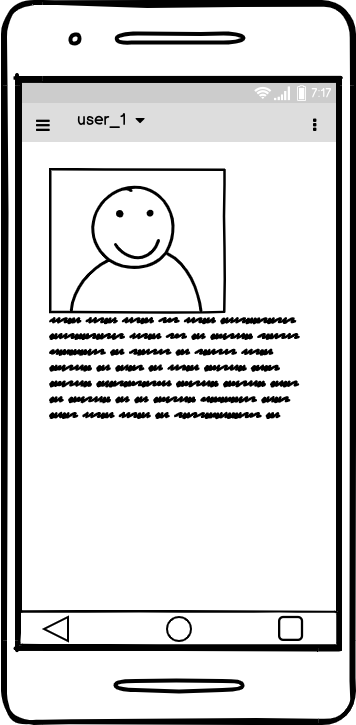
\includegraphics[width=\linewidth]{figs/user_1.png}
        \caption{User Profile} \label{fig:x_a}
    \end{subfigure}
    \hspace*{\fill}
    \begin{subfigure}{0.3\textwidth}
        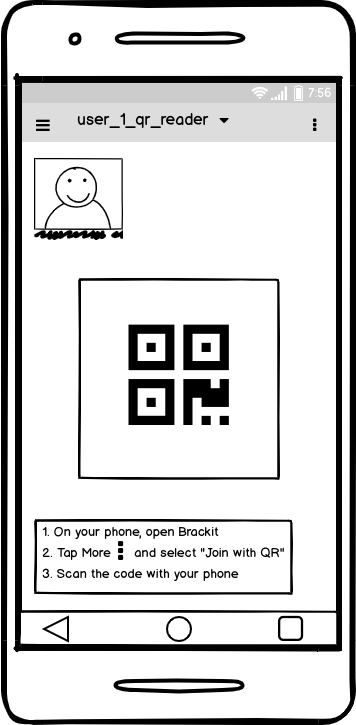
\includegraphics[width=\linewidth]{figs/user_1_qr_reader.png}
        \caption{QR Reader} \label{fig:x_b}
    \end{subfigure}
    \hspace*{\fill}
    \begin{subfigure}{0.3\textwidth}
        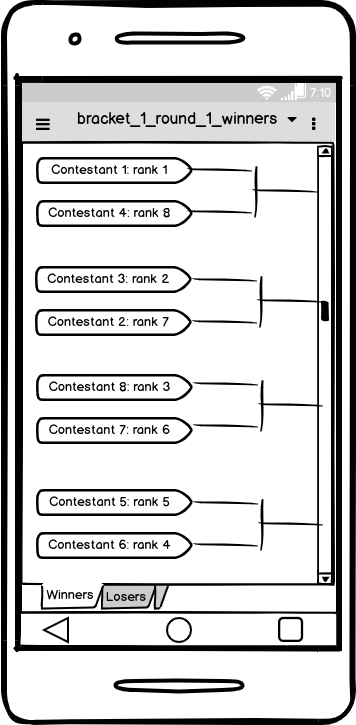
\includegraphics[width=\linewidth]{figs/bracket_1_round_1_winners.png}
        \caption{Vertical Bracket Visualization} \label{fig:x_c}
    \end{subfigure}
    \begin{subfigure}{1\textwidth}
        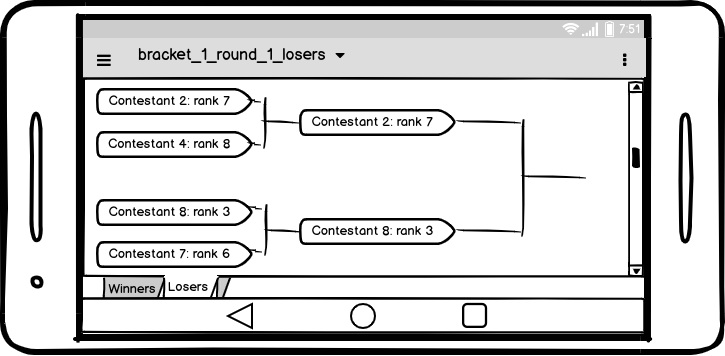
\includegraphics[width=\linewidth]{figs/bracket_1_round_2_losers.png}
        \caption{Horizontal Bracket Visualization} \label{fig:x_c}
    \end{subfigure}
\end{figure*}

% \bibliography{mybib.bib}
% \bibliographystyle{plain}
\end{document}